\begin{sidewaysfigure*}
    \thisfloatpagestyle{mylandscape}%
    \rotatesidewayslabel%
\centering
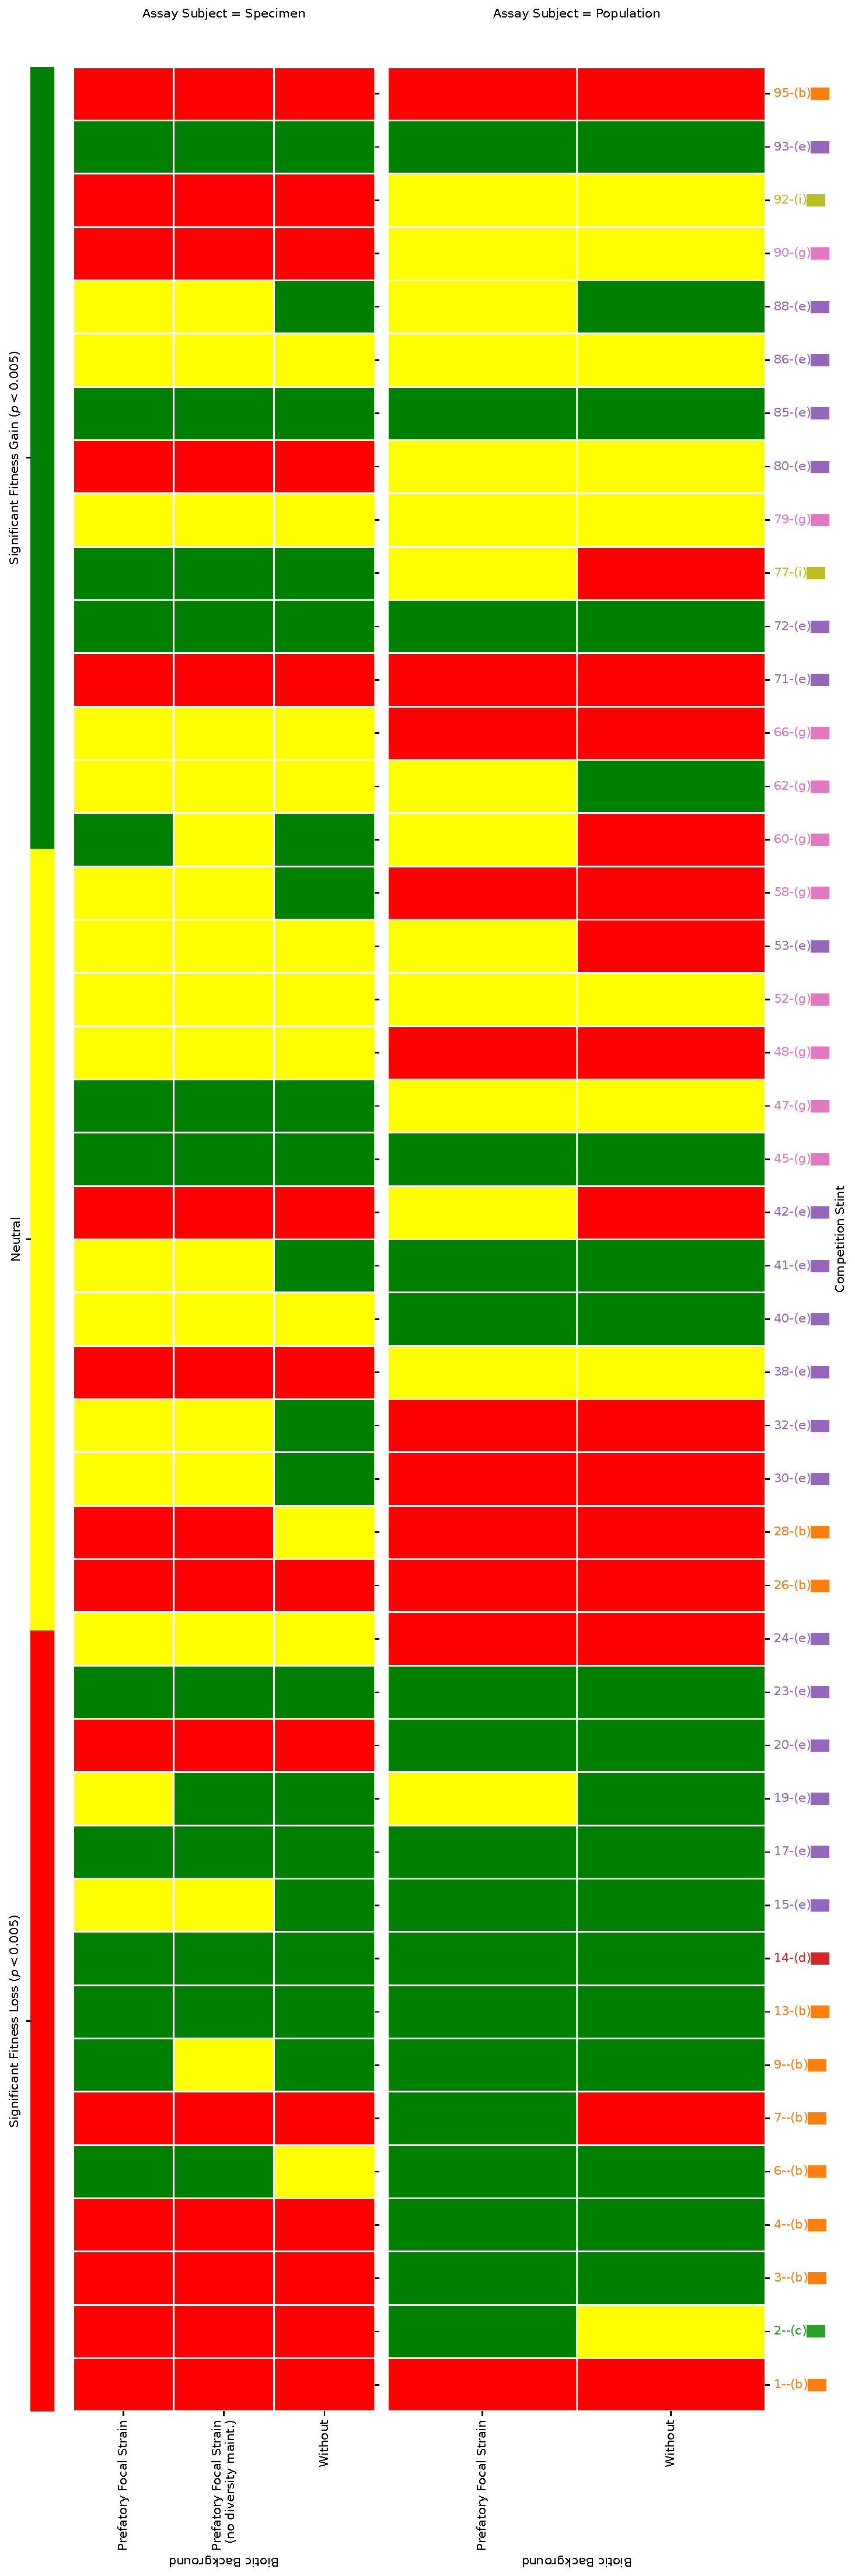
\includegraphics[width=\linewidth]{{submodule/dishtiny/binder/bucket=prq49/a=adaptation_assays+endeavor=16/teeplots/a=baselinecontrol+hue=fitness-gain-or-loss+viz=facet-heatmap+x=biotic-background+y=competition-stint+ext=}}

\caption{
\textbf{Adaptation assay outcomes.}
\footnotesize
Summary of biotic background control adaptation assay outcomes for sampled representative specimen (top) and population-level adaptation (bottom).
Color coding and parentheticals of stint labels correspond to qualitative morph codes described in Table \ref{tab:morph_descriptions}.
See Figure \ref{fig:adaptation_assay_cartoon} for explanation of competition biotic backgrounds.
}
\label{fig:baseline_fitness_gain_or_loss}
\end{sidewaysfigure*}
